\documentclass[10pt]{article}
\usepackage[usenames]{color} %used for font color
\usepackage{amssymb} %maths
\usepackage{amsmath} %maths
\usepackage[utf8]{inputenc} %useful to type directly diacritic characters
\usepackage{tikz}
\usetikzlibrary{external}
\usetikzlibrary{quotes,angles}
\usetikzlibrary{decorations.markings}
\usepackage{sansmath}
\usetikzlibrary{shadings,intersections}

\begin{document}
\[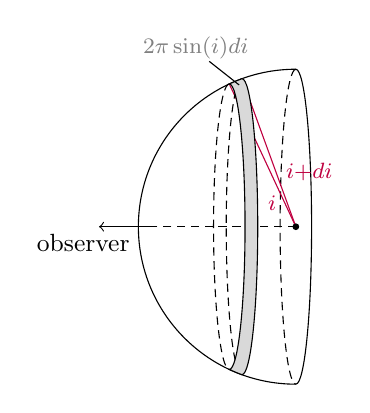
\begin{tikzpicture}
  \coordinate (O) at (0,0);

  % ball background color
  %\shade[ball color = blue, opacity = 0.2] (0,0) circle [radius = 2cm];

  % hemisphere
  \draw[black] (0,2cm) arc [start angle = 90, end angle = 270,
    x radius = 2cm, y radius = 2cm];
  \draw[densely dashed] (0cm,2cm) arc [start angle = 90, end angle = 270,
    x radius = 2mm, y radius = 2cm];
  \draw (0cm,2cm) arc [start angle = 90, end angle = -90,
    x radius = 2mm, y radius = 2cm];

  % radius
  \draw [purple] (O) to (110:2cm) node at (.17,.7) {\footnotesize $i$+$di$}; 
  \draw [purple] (O) to (115:2cm) node at (-.3,.3) {\footnotesize $i$}; 
  %\draw (O) ++ (110:2cm) arc [start angle = 110, end angle = 115,
  %  x radius = 2cm, y radius = 2cm];

  
  \draw[densely dashed] (O) -- (-1.8cm,0);
  \draw [->] (O)++(-1.8cm,0) -- (-2.5cm,0) node at (-2.7,-.2)  {\small observer};

  
  % label of ball center point
  \filldraw (O) circle (1pt);

  % annulus
  \draw[densely dashed] (O) ++ (110:2cm) arc [start angle = 90, end angle = 270,
    x radius = 2mm, y radius = 2cm*sin(110)];
  %\draw [gray] (O) ++ (110:2cm) arc [start angle = 90, end angle = -90,
  %  x radius = 2mm, y radius = 2cm*sin(110)];
  \draw[densely dashed] (O) ++ (115:2cm) arc [start angle = 90, end angle = 270,
    x radius = 2mm, y radius = 2cm*sin(115)];
  %\draw [gray] (O) ++ (115:2cm) arc [start angle = 90, end angle = -90,
  %  x radius = 2mm, y radius = 2cm*sin(115)];

  \draw [fill = gray!30] (O) ++ (110:2cm) arc [start angle = 90, end angle = -90,
    x radius = 2mm, y radius = 2cm*sin(110)]
    arc [start angle = -110, end angle = -115,
    x radius = 2cm, y radius = 2cm]
    arc [start angle = -90, end angle = 90,
    x radius = 2mm, y radius = 2cm*sin(115)]
    arc [start angle = 115, end angle = 110,
    x radius = 2cm, y radius = 2cm];

   % cut of ball surface  % label of cut of ball surface
  \draw (-1.1,2.1) -- (-0.72,1.8) node at (-1.27,2.27) [gray] {\footnotesize $2\pi\sin(i)di$};


\end{tikzpicture}
\]
\end{document}